%% -*- latex -*-
\documentclass[12pt]{tufte-handout}

\usepackage[british]{babel}
\usepackage{booktabs}
\usepackage{tikz}
\usetikzlibrary{calc,shapes.geometric} 
\usepackage{tikz-timing}
\usepackage{minted}
\usepackage{graphicx}
\usepackage{natbib}
\usepackage{siunitx}
\usepackage[theorems,skins]{tcolorbox}
\tcbset{enhanced}
\newtcbtheorem{exercise}{Exercise}{drop fuzzy shadow}{ex}
\newtcbtheorem{question}{Question}{drop fuzzy shadow}{q}
\usepackage{amssymb}

\title{LPC4088 Timer Interrupts\\
Light Characteristics\\
\small{CM0506 Small Embedded Systems}}
\author{Dr Alun Moon}
\date{Seminar 2a}

\definecolor{code}{wave}{602}
%\definecolor{cmd}{wave}{528}
\definecolor{cmd}{named}{SkyBlue}

\hypersetup{colorlinks, urlcolor = DarkRed}

\begin{document}
\maketitle
\section{Navigation Lights}
\newthought{Maritime navigation lights have very defined
  characteristics.}  These are the rate and pattern of flashes.  These
are defined in IALA Recomendation E-110 \citep{iala-e}.  A summary is
in Wikipedia at
\url{https://en.wikipedia.org/wiki/Light_characteristic}.

\section{Types of flashes}
A summary of the characteristics is given below.  There are some
simplifications I've made.
\subsection{Occulting}
\paragraph{An Occulting light shows a steady light, interrupted by
  short periods of darkness.}  The period of light is longer than the
period of dark.
\newthought{Single-occulting light} The length of the light is three
times the length of the dark period.  The overall period of the light
is at least 2 seconds.

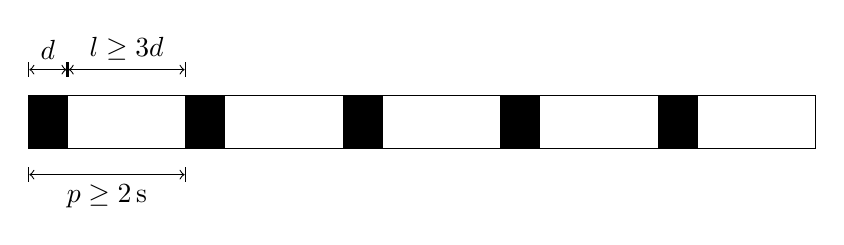
\begin{tikzpicture}[scale=2]%occulting
  \foreach \n in {0,...,4} {
    \draw (\n,0) rectangle +(1,1/3);
    \fill (\n,0) ++(0,0) rectangle +(1/4,1/3);
  }
  \draw[|<->|] (0,1/2)--node[above]{$d$}(1/4,1/2);
  \draw[|<->|] (1/4,1/2)--node[above]{$l\ge 3d$}(1,1/2);
  \draw[|<->|] (0,-1/6)--node[below]{$p\ge\SI{2}{s}$}(1,-1/6);
\end{tikzpicture}
\[
 l \ge 3d \hspace{1in}  p\ge\SI{2}{s}
\]

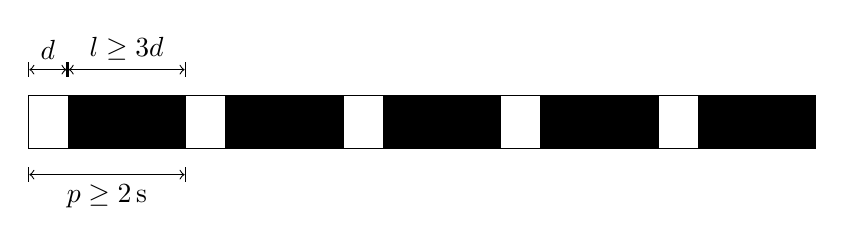
\begin{tikzpicture}[scale=2]%flashing
  \foreach \n in {0,...,4} {
    \draw (\n,0) rectangle +(1,1/3);
    \fill (\n,0) ++(1/4,0) rectangle +(3/4,1/3);
  }
  \draw[|<->|] (0,1/2)--node[above]{$d$}(1/4,1/2);
  \draw[|<->|] (1/4,1/2)--node[above]{$l\ge 3d$}(1,1/2);
  \draw[|<->|] (0,-1/6)--node[below]{$p\ge\SI{2}{s}$}(1,-1/6);
\end{tikzpicture}

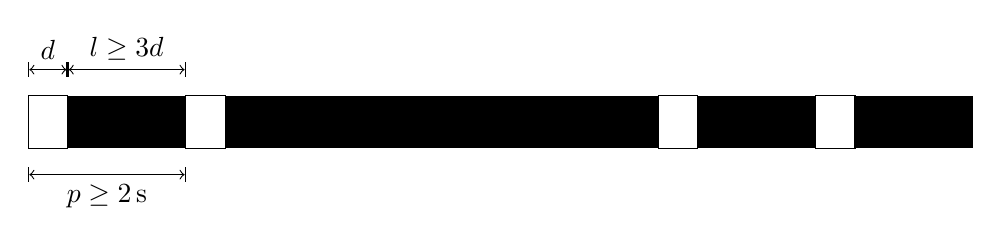
\begin{tikzpicture}[scale=2]%group flashing
  \fill (0,0) rectangle +(6,1/3);
  \foreach \n in {0,1,4,5} {
    \draw[fill=white] (\n,0) rectangle +(1/4,1/3);
    %%%%%\fill (\n,0) ++(1/4,0) rectangle +(3/4,1/3);
  }
  \draw[|<->|] (0,1/2)--node[above]{$d$}(1/4,1/2);
  \draw[|<->|] (1/4,1/2)--node[above]{$l\ge 3d$}(1,1/2);
  \draw[|<->|] (0,-1/6)--node[below]{$p\ge\SI{2}{s}$}(1,-1/6);
\end{tikzpicture}

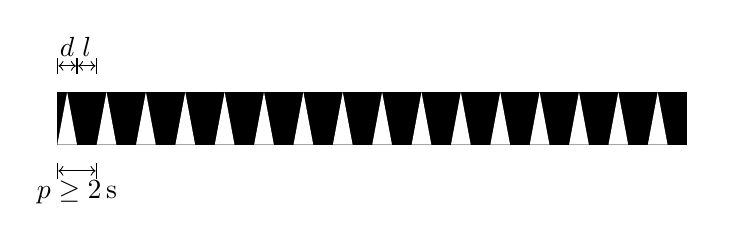
\begin{tikzpicture}[scale=2]%quick flashing
  \fill (0,0) rectangle +(4,1/3);
  \foreach \n in {0,0.25,...,4} {
    \fill[white] (\n,0) -- +(1/16,1/3) -- +(2/16,0) -- cycle;
  }
  \draw[|<->|] (0,1/2)--node[above]{$d$}(1/8,1/2);
  \draw[|<->|] (1/8,1/2)--node[above]{$l$}(1/4,1/2);
  \draw[|<->|] (0,-1/6)--node[below]{$p\ge\SI{2}{s}$}(1/4,-1/6);
\end{tikzpicture}

\begin{description}
\item[Occulting] period not less than \SI{2}{s} light at least 3 times
  greater than the dark
\item[Isophase]  period not less than \SI{2}{s} light and dark equal
\item[Long flash] light greater than \SI{2}{s}, dark 3 times longer
  than light
\item[Flashing] period not less than \SI{2}{s} (rate less than 50 per minute), dark 3 times longer
  than light
\item[Quick flashing] 60 flashes per minute
\item[Very Quick flash] 120 flashes per minute
\end{description}

Period is split into 4 sections, so period has to be a multiple of 4.
For $\SI{1.2}{s} \equiv \SI{1200}{ms} \therefore \frac{1}{4} \equiv
\SI{300}{ms}$.
For 120 fpm , period is \SI{0.5}{s} or \SI{500}{ms}, flashes are
almost isophase so light \SI{200}{ms} and dark \SI{300}{ms} works.

\section{Prescaler}
The timer increments the timer-counter for every $P_r+1$ counts of the
Peripheral Clock, where $P_r$ is the value of the prescale register.

The Peripheral Clock ticks at a \SI{60}{\mega\hertz} rate.  With
$P_r=59$ the timer ticks at a rate of \SI{1}{\mega\hertz}, or the
timer counts in \si{\micro\second}.  If $P_r=\num{59999}$ the timer
counts in \si{\milli\second}


\bibliography{lpc4088}
\bibliographystyle{plainnat}
\end{document}

%% Local Variables:
%% mode: reftex
%% mode: auto-fill
%% mode: flyspell
%% mode: tabkey2
%% End:
